\documentclass{article}
\usepackage{graphicx} % Required for inserting images
\usepackage{amssymb}
\usepackage{amsmath}
\usepackage{geometry} 
\geometry{left=2.5cm,right=2.5cm,top=2.5cm,bottom=2.5cm}

\title{Estimação de $\pi$ através do algoritmo de Monte Carlo}

\author{Rennisson Davi D. Alves - 13687175}
\date{Abril de 2023}

\begin{document}

\maketitle

    \section{Introdução}
    \paragraph{} O objetivo deste trabalho é tentar estimar a área do círculo unitário através do método de Monte Carlo. Para tratar deste problema e chegar no valor de $\pi$ (número para o qual a área do circulo unitário converge) através do método computacional de Monte Carlo vamos primeiro considerar que o sorteio de pontos dentro do intervalo (-1, 1) para todo x e y segue uma distribuição binomial. E após isso, vamos aproximar a binomial através da distribuição normal, a fim de facilitar alguns cálculos.
    \paragraph{} Como ferramenta, foi utilizada a linguagem de programação python com sua biblioteca numpy para desenvolvimento do algoritmo de Monte Carlo e realização dos experimentos. Para o seed do random, foi utilizado o NUSP 13687175. 
    
    \section{Aproximação da binomial pela distribuição normal}
    
    \paragraph{} Como dissemos anteriormente, o sorteio de pontos segue uma distribuição binomial. A equação da circunferência é $x^2 + y^2 \le 1$ e a utilizaremos para analisar se determinado ponto está dentro ou não da circunferência unitária.

    \paragraph{} Não é difícil perceber que para nos aproximarmos o máximo possível do resultado esperado precisaremos de uma imensa quantidade de pontos, nesse caso, queremos uma precisão de 99.5\%. E calcular probabilidade para tamanha quantidade de eventos não é tarefa fácil quando usamos a distribuição binomial.

    \paragraph{} Para simplificar o problema, podemos aproximar a binomial através da distribuição normal. O maior trabalho aqui é a manipulação algébrica para realizar essa transformação, porque depois de feita só precisamos substituir valores e encontrar valor-z correspondente na tabela normal.

    \paragraph{} De início, nossa variável X (pontos dentro da circunferência unitária) segue uma distribuição binomial com parâmetros n, números de eventos, e p, probabilidade do ponto escolhido estar na região \begin{math} x^2 + y^2 \le 1 \end{math}. Tal distribuição é denotada por $X \sim bin(n, p)$.

    \paragraph{}
    Em geral, a normal tem como parâmetros a esperança (ou média) E(X) e sua variância Var(X), mais comumente representados por \begin{math} \mu\ e\ \sigma^2 \end{math}, respectivamente. A média da binomial é E(X)=np e sua variância é Var(X)=np(1-p). Para que ocorra a aproximação entre as duas distribuições basta que passemos a esperança e a variância da binomial como os respectivos parâmetros da normal, ficando então \begin{math} \mu = np\ e\ \sigma = np(1-p) \end{math}. Para não haver confusão, agora a nossa variável normalizada é \begin{math} Y \sim N(\mu,\sigma) \end{math}.

    \section{Estimação dos parâmetros}
    \paragraph{} Não temos ainda os valores exatos de $\mu\ e\ \sigma$, então precisamos estimá-los.
    \paragraph{} Para o estimador $\widehat{p}$, podemos observar que a circunferência está contida no quadrado de lado 2r (como r=1, o quadrado tem lado 2). Desse modo, deduzimos que a probabilidade de um ponto estar dentro da circunferência é  $\widehat{p} = \frac{Área\ do\ círculo}{Área\ do\ quadrado} = \frac{\pi r^2}{(2r)^2} = \frac{\pi}{4}$.
    \paragraph{} Com esse estimador já podemos trabalhar um pouco mais com a nossa distribuição para descobrirmos o erro $\varepsilon$ que podemos cometer e conseguirmos dimensionar o número n mínimo de pontos necessários para uma boa aproximação.
    \begin{gather*}
        P(|\widehat{p} - p| < \varepsilon) \ge \gamma \\ \\
        P \biggl( \frac{-\varepsilon}{\frac{\sigma}{\sqrt{n}}} < \frac{\widehat{p} - p}{\frac{\sigma}{\sqrt{n}}} < \frac{\varepsilon}{\frac{\sigma}{\sqrt{n}}} \biggl) =
        P \biggl( \frac{-\sqrt{n}\varepsilon}{\sigma} < Z < \frac{\sqrt{n}\varepsilon}{\sigma} \biggl) = P \biggl( -z_\gamma < Z < z_\gamma \biggl)\ge \gamma
    \end{gather*}

    \paragraph{} Note que $z_\gamma = \frac{\sqrt{n}\varepsilon}{\sigma}$. Como foi exigida uma precisão $\gamma = 99.95\%$ para o nosso intervalo de confiança, temos que $z_\gamma = 3.27$, pela tabela normal padronizada. Dessa mesma relação, vamos estimar n:

    \begin{gather*}
        z_\gamma = \frac{-\sqrt{n}\varepsilon}{\sigma} \Longrightarrow n = \frac{z_\gamma^2 \sigma^2}{\varepsilon^2}
    \end{gather*}

    \paragraph{} Já temos $z_\gamma\ e\ \sigma$. Vamos procurar $\varepsilon$\ agora:
    
    \begin{gather*}
        \frac{|\widehat{\pi}-\pi|}{\pi} \le 0.0005 \\
    \end{gather*}

    \paragraph{} Lembre que $\widehat{\pi} = 4\cdot T(x_i) = 4\cdot 1(x^2+y^2\le 1)$. Então
    
    \begin{gather*}
        \frac{|4\cdot T(x_i)-\pi|}{\pi} =
        4\cdot \frac{|T(x_i)-\pi|}{\pi} \le 0.0005 \\
    \end{gather*}

    \paragraph{} Realizamos alguns teste de antemão e vamos utilizar a média dos $\pi$ encontrados nos experimentos realizados, apenas para termos um ponto de partida.

    \begin{center}
        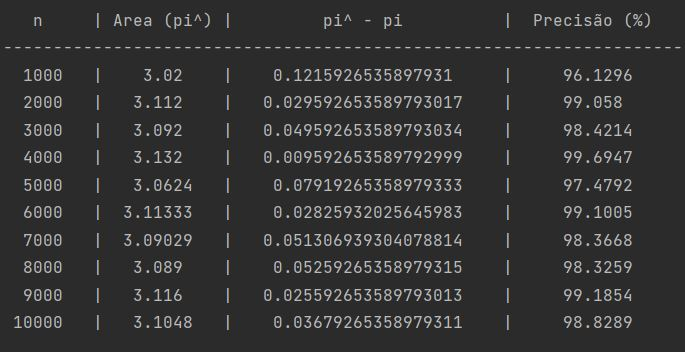
\includegraphics[width=0.8\textwidth]{experimento_inicial}\\
        \caption{Primeiros experimentos}
    \end{center}
    
    \begin{gather*}
        \frac{|3.093182 - \pi|}{\pi} \le 0.000125 \\
        |3.093182 - \pi| \le 0.000125 \pi \Longrightarrow \varepsilon = 0.000125 \widehat{\pi} = 0.00038665
    \end{gather*}

    \paragraph{} Com o $\varepsilon$ definido, basta substituir os valores e encontramos o n procurado:

    \begin{gather*}
        n = \frac{z_\gamma^2 \sigma^2}{\varepsilon^2} = \frac{z_\gamma^2 \cdot (\widehat{p}(1-\widehat{p}))}{\varepsilon^2} = \frac{3.27^2 (\frac{\pi}{4}(1-\frac{\pi}{4}))}{0.00038665^2} = 12055432.3989
    \end{gather*}

    \paragraph{} Logo, se utilizarmos um n $\ge$ 12055433, vamos chegar a um valor próximo o suficiente do $\pi$ real.

    \section{O algoritmo de Monte Carlo, experimentos e resultados}
    \paragraph{} O algoritmo de Monte Carlo é uma técnica computacional desenvolvida para testes e aproximação de resultados de certos problemas. É uma ferramenta de inferência estatística utilizada geralmente em problemas muito complexos que só conseguem ser verificados através da ajuda dos computadores.
    \paragraph{} É justamente isso que precisamos neste caso. O problema em si não parece complexo, mas a verificação de seus resultados pode ser bastante trabalhosa. Fica mais clara ainda a sua necessidade se prestarmos atenção na última seção: para atingir um resultado satisfatório precisamos de um n maior que 7.000.000. Inviável sortear manualmente tal numero de pontos e verificar se cada um deles está na circunferência unitária. Por isso deixamos esse trabalho nas mãos do algoritmo de Monte Carlo. Deixamos que ele sorteie todos os pontos e verifique se cada ponto está ou não na circunferência unitária. Ao fim de cada experimento ele retorna a frequência de pontos dentro da circunferência, que se aproxima da área do próprio círculo a medida que vamos aumentando a nossa amostra de pontos.
    \paragraph{} Feita a análise dos parâmetros, vamos verificar os resultados obtidos através do algoritmo de Monte Carlo.
    
    \begin{center}
        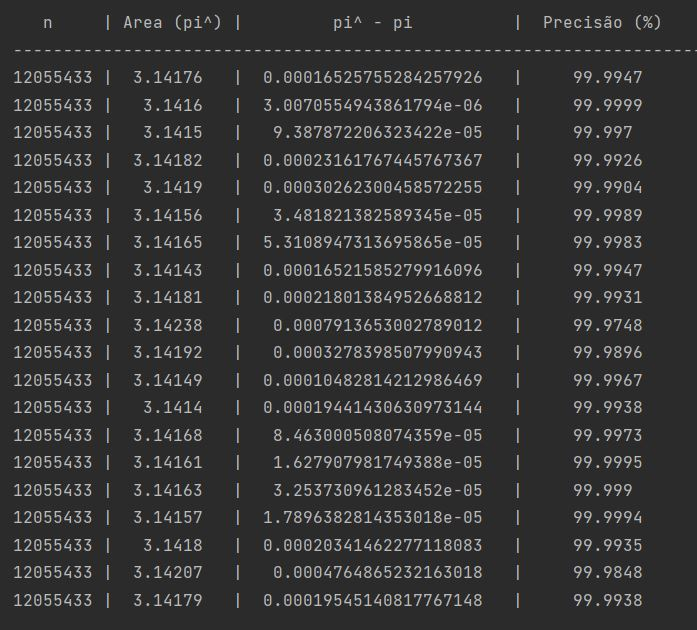
\includegraphics[width=0.6\textwidth]{experimento_final1}\\
        \caption{Experimentos com n=12055433}

        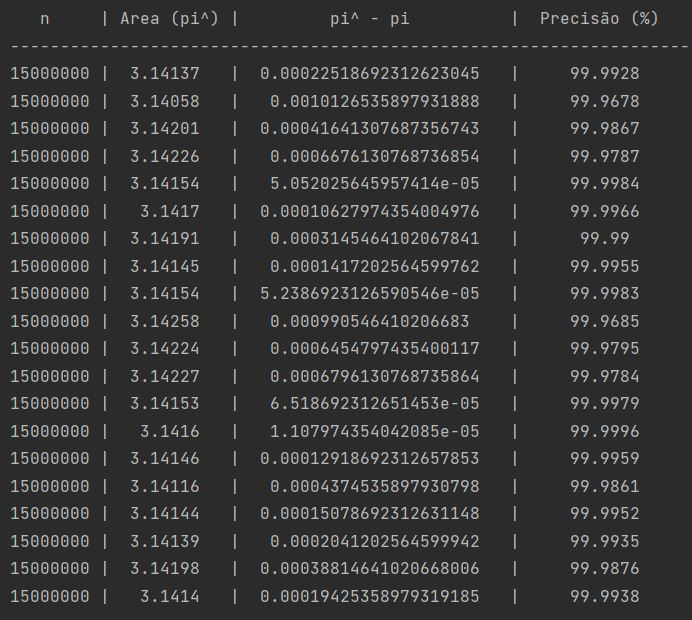
\includegraphics[width=0.6\textwidth]{experimento_final2}\\
        \caption{Experimentos com n=15000000}
    \end{center}

    \paragraph{} Observe que os resultados dos experimentos com n maior ou igual ao n estimado pelos processos algébricos das seções anteriores são excelentes. À exceção de um ou outro teste, quase todos os experimentos atingiram a precisão desejada. Tal desempenho dos experimentos realizados reforçam o caráter preciso e útil do método de Monte Carlo.

\end{document}
